\documentclass[b5paper,xelatex,ja=standard,10pt]{bxjsarticle}
\usepackage{mystyle}  % export TEXINPUTS="./;../sty/;"
\graphicspath{{../images/}}

\usepackage{listings}
\lstset{  % グローバル設定
  columns=fixed,  % 等幅
  basewidth=0.5em,  % 字間詰め
  lineskip=-3pt,  % 行間詰め
  % フォント設定
  basicstyle={\ttfamily\small\color{DarkGray}},  % 全体設定
  keywordstyle=[1]{\color{RoyalBlue}},  % kewords[1]の設定 (Python だと予約語)
  keywordstyle=[2]{\color{VioletRed}},  % kewords[2]の設定 (Python だと組み込み関数)
  stringstyle={\color{FireBrick}},  % 文字列リテラルの設定
  commentstyle={\color{SeaGreen}},  % コメントの設定
}

\renewcommand{\footnoterule}{%
  \kern -5pt
  \color{DarkGray}
  \hrule width \textwidth height 1pt
  \kern 4.7pt
}

\makeatletter
\renewcommand*\l@section{\@dottedtocline{1}{0.0em}{4.0em}}
\makeatother

\usepackage{eso-pic}

\newcommand\BackgroundPic{%
\put(0,0){%
\parbox[b][\paperheight]{\paperwidth}{%
\vfill
\centering
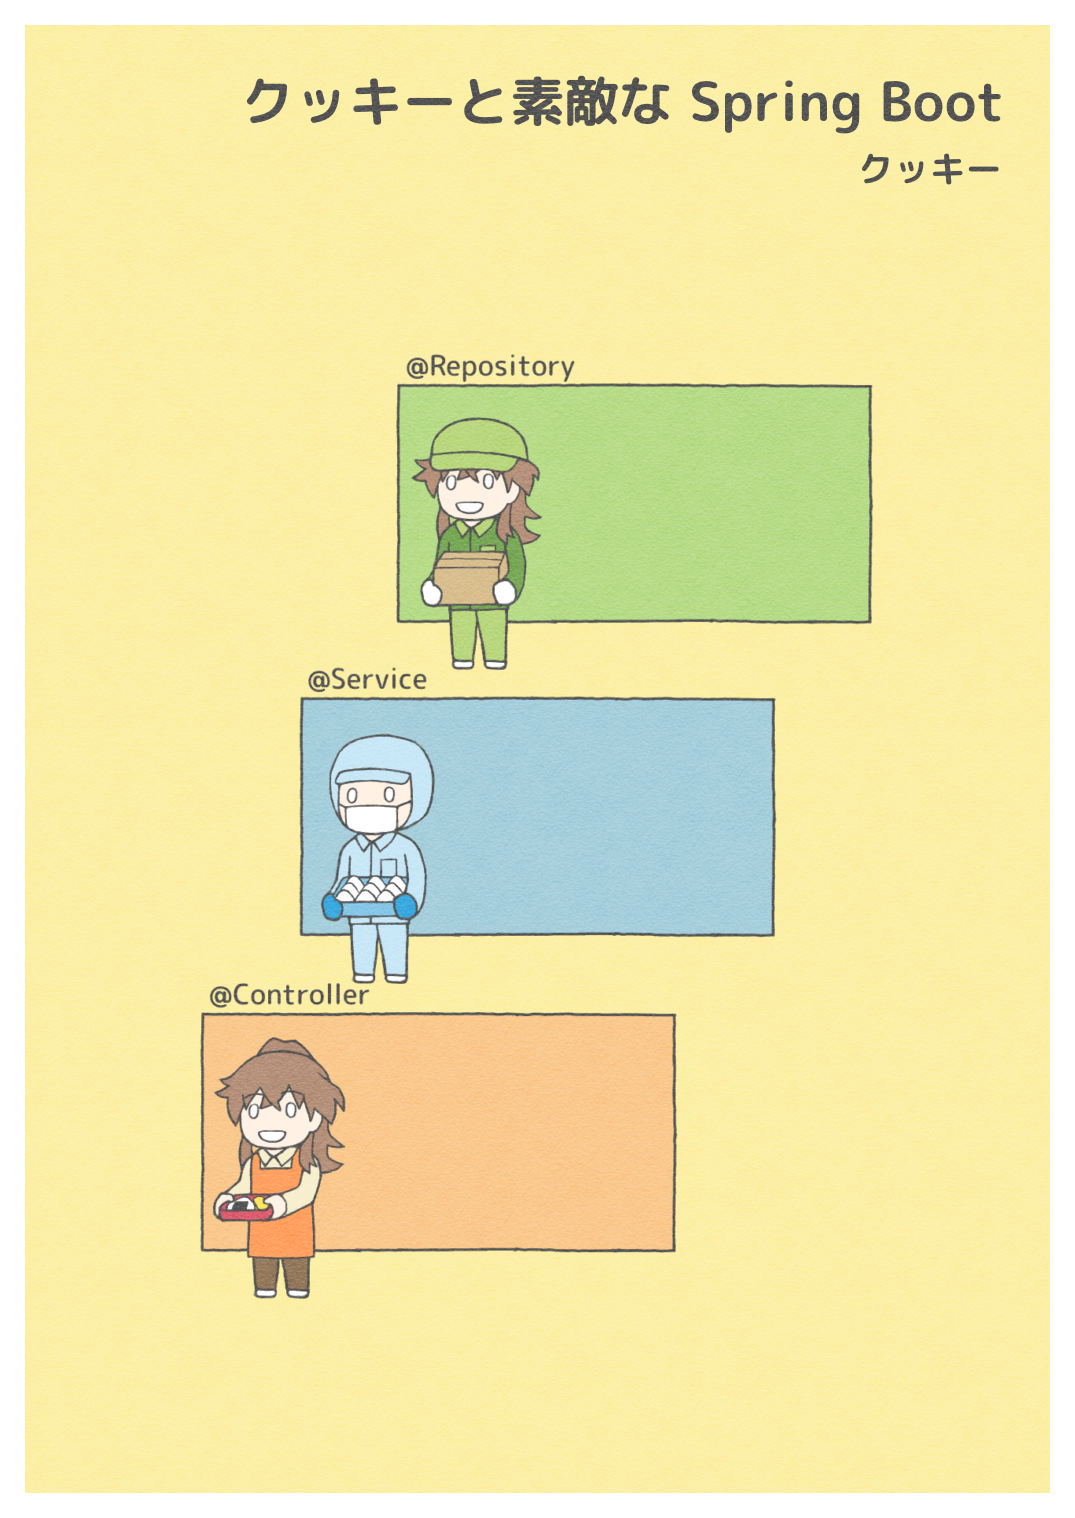
\includegraphics[width=0.99\paperwidth,height=0.99\paperheight,%
keepaspectratio]{cover.png}%
\vfill
}}}



\begin{document}

\AddToShipoutPicture*{\BackgroundPic}
\begin{titlepage}
\ 
\end{titlepage}

% 地の文の文字色をグレーに変更する
\addfontfeatures{Color=DarkGray}
\addCJKfontfeatures{Color=DarkGray}

%\part*{クッキーと素敵な Spring Boot}

\begin{spacing}{1.0}
\textbf{\tableofcontents}
\end{spacing}


\section*{まえがき}
\addcontentsline{toc}{section}{まえがき}
%\addcontentsline{toc}{section}{\protect\numberline{\null}まえがき}
\vspace{3pt}

以下の JDK を使用しています。
\begin{itemize}
\item openjdk 11.0.13 2021-10-19
\item OpenJDK Runtime Environment Temurin-11.0.13+8 (build 11.0.13+8)
\item OpenJDK 64-Bit Server VM Temurin-11.0.13+8 (build 11.0.13+8, mixed mode)
\end{itemize}

以下のパッケージを使用しています。
\begin{itemize}
\item Spring Boot 2.6.1
\end{itemize}

お気付きの点がありましたらこの原稿のリポジトリの Issues までお願いいたします。

https://github.com/CookieBox26/notes/issues


\newcounter{mycounter}
\stepcounter{mycounter}
\newcommand*{\mysectiontitle}{クッキー、Spring Boot 開発に参加する}
\section*{第{\themycounter}話 \, \mysectiontitle}
\addcontentsline{toc}{section}{\numberline {第{\themycounter}話}\mysectiontitle}
\vspace{3pt}

\begin{SERIFU}[colback=PaleIris, colbacktitle=PaleIris2]{kazusa_1.png}
Spring Boot (Java)による REST API 開発に参加することになりました。Python でならいくつかのやり方で REST API を実装したことがありますが、Spring Boot は触ったことがありません。そもそも Java での開発も初めてに等しいです。Java モジュールに数行の修正 PR をしたことは何度かありますが、機能追加をするなどは経験がないので、Java における開発プラクティスの知見もまるでありません。C\# での開発経験はありますが昔すぎて記憶が……。
\end{SERIFU}

\begin{SERIFU}[colback=PaleIris, colbacktitle=PaleIris2]{kazusa_2.png}
……まあしかし、REST API であるならばコードをみれば何が何なのかは概ねわかるでしょう。今回の私のタスクは何もスクラッチで REST API を構築することではありません。{\addCJKfontfeatures{Color=VioletRed}{\addfontfeatures{Color=VioletRed}現在既に「弁当」を返却しているベントウAPIがあり、リクエストに応じてその「弁当」に「卵焼き」を追加する}}だけです。外部 API から新たに「卵」を取り寄せる必要はありますが――。
\end{SERIFU}

\begin{SERIFU}[colback=PaleIris, colbacktitle=PaleIris2]{kazusa_0.png}
ともかく適当なソースファイルをみてみましょう――どのファイルも1行目に
\begin{CODE}[title=\texttt{src/main/java/com/example/bentou/BentouApplication.java}]
\begin{lstlisting}[language=java]
package com.example.bentou;
\end{lstlisting}
\end{CODE}
などとありますね。これは「このソースファイル内に定義されているクラスは com.example.bentou なるパッケージに所属しています」という意味ですか。クラスを適宜パッケージに整理せよということですね。
\end{SERIFU}

\begin{SERIFU}[colback=PaleIris, colbacktitle=PaleIris2]{kazusa_0.png}
では、HTTP リクエストを受け取るハンドラはどこにあるのでしょうか?  現在の仕様書によると {\addfontfeatures{Color=FireBrick}/bentou} なるエンドポイントに HTTP GET することで「弁当」が返却されるはずですが……あっ、このクラスでしょうか。
\begin{CODE}[title=\texttt{src/main/java/com/example/bentou/BentouController.java}]
\begin{lstlisting}[language=java,emph={@RestController,@Autowired,@Qualifier,@GetMapping},emphstyle=\color{VioletRed}]
package com.example.bentou;

import org.springframework.beans.factory.annotation.Autowired;
import org.springframework.beans.factory.annotation.Qualifier;
import org.springframework.web.bind.annotation.GetMapping;
import org.springframework.web.bind.annotation.RestController;

@RestController
public class BentouController {
    private final OnigiriService service;

    @Autowired
    public BentouController(@Qualifier("tuna") OnigiriService service) {
        this.service = service;
    }

    @GetMapping("/bentou")
    public Onigiri provide() {
        Onigiri onigiri = this.service.provideOnigiri();
        return onigiri;
    }
}
\end{lstlisting}
\end{CODE}
{\addfontfeatures{Color=VioletRed}@GetMapping}({\addfontfeatures{Color=FireBrick}"/bentou"}) が付加されたメソッド(Python でいうデコレータのようですが――?)がリクエストを受け取っておにぎりを返却しているようにみえます。このメソッドがリクエストハンドラとみていいでしょう。
\end{SERIFU}


\stepcounter{mycounter}
\renewcommand*{\mysectiontitle}{クッキー、最大の謎に直面する}
\section*{第{\themycounter}話 \, \mysectiontitle}
\addcontentsline{toc}{section}{\numberline {第{\themycounter}話}\mysectiontitle}


\begin{SERIFU}[colback=PaleIris, colbacktitle=PaleIris2]{kazusa_0.png}
リクエストハンドラがわかればリクエストに応じて返却フィールドを追加する変更は実装できそうです。
\end{SERIFU}

\begin{SERIFU}[colback=PaleIris, colbacktitle=PaleIris2]{kazusa_1.png}
……しかし、リクエストハンドラをもつ BentouController クラスがどこでインスタンス化されているのかさっぱりわかりません。リポジトリを grep してもそれらしき箇所がありません。BentouController クラスにはコンストラクタもあるようですし、やはりこれはインスタンス化して利用するものでしょう。であれば、何がどうなって――
\end{SERIFU}


\stepcounter{mycounter}
\renewcommand*{\mysectiontitle}{クッキー、Controller の単体テストで行き詰まる}
\section*{第{\themycounter}話 \, \mysectiontitle}
\addcontentsline{toc}{section}{\numberline {第{\themycounter}話}\mysectiontitle}


\stepcounter{mycounter}
\renewcommand*{\mysectiontitle}{クッキー、RestTemplate の利用に行き詰まる}
\section*{第{\themycounter}話 \, \mysectiontitle}
\addcontentsline{toc}{section}{\numberline {第{\themycounter}話}\mysectiontitle}


\stepcounter{mycounter}
\renewcommand*{\mysectiontitle}{クッキー、Service の単体テストで行き詰まる}
\section*{第{\themycounter}話 \, \mysectiontitle}
\addcontentsline{toc}{section}{\numberline {第{\themycounter}話}\mysectiontitle}


\stepcounter{mycounter}
\renewcommand*{\mysectiontitle}{クッキー、サーキットブレーカーに嫌われる}
\section*{第{\themycounter}話 \, \mysectiontitle}
\addcontentsline{toc}{section}{\numberline {第{\themycounter}話}\mysectiontitle}


\stepcounter{mycounter}
\renewcommand*{\mysectiontitle}{クッキー、接続プールが不足する}
\section*{第{\themycounter}話 \, \mysectiontitle}
\addcontentsline{toc}{section}{\numberline {第{\themycounter}話}\mysectiontitle}


\stepcounter{mycounter}
\renewcommand*{\mysectiontitle}{クッキー、メトリクスを隠される}
\section*{第{\themycounter}話 \, \mysectiontitle}
\addcontentsline{toc}{section}{\numberline {第{\themycounter}話}\mysectiontitle}


\stepcounter{mycounter}
\renewcommand*{\mysectiontitle}{クッキーと素敵な Spring Boot}
\section*{第{\themycounter}話 \, \mysectiontitle}
\addcontentsline{toc}{section}{\numberline {第{\themycounter}話}\mysectiontitle}


\addcontentsline{toc}{section}{参考文献}
\begin{thebibliography}{99}
    \bibitem{mockito_stubbing_consecutive_calls} \url{https://javadoc.io/doc/org.mockito/mockito-core/4.0.0/org/mockito/Mockito.html#10}
\end{thebibliography}


% \vspace{5pt}
% \noindent つづかない


\end{document}
